
\section{Recurrent Neural Networks}
If we feed a feed forward network with a string, it produces a binary vector as an output.
Consequently, the order of the words are lost.
A recurrent layer re-introduces the words order into the networks internal.
Recurrent layer outputs that are calculated during propagation of an input $n$, are used to calculate the same input $n+1$. 
Compared to an feed forward network, we distinguish inputs chronologically by an index $t: x_{t-1},x_t, x_{t+1}$.
In addition, there is a second matrix $U$, such that values can be sent to the next layer:
\begin{equation}
    \sigma(Ax_t+Ux_{t-1}+b)
\end{equation}
\cite{haralambous_course_2024}
\ac{RNN} can only process word by word and this is why they are operating very slow, compared to transformer, that are able to process a complete sentence 

\section{Transformer Models}
A Deep Neural Network, that identifies contextual relationships within sequential data by using a self-attention mechanism is called a Transformer as Vaswani et al \cite{vaswani_attention_2023} introduced in their famous paper.
Transformer Models as GPT and BERT have been trained as language models.
During this task, the models have been trained on a large amount of raw text in a self-supervised way.
In self-supervised learning, the models inputs are used to automatically compute the objectives.
This implies that the data does not require a human labelling.
Even though it isn't very helpful for specific practical tasks, as this kind of model builds a statistical understanding of the language it has been trained on.
This is why the general pretrained model undergoes a procedure known as transfer learning.
This approach fine-tunes the model in a supervised way on a given task, where human annotated labels are used.\cite{Huggingface}

During a transfer learning task, the model is pretrained from the scratch, the weights are randomly initialized and the training starts without any prior knowledge, further a very large amount of data is used and the training can take up to several weeks.
After the model has been pretrained, a fine-tuning tasked is performed, where a additional training with a dataset specific to the required task is performed.
For example, a pretrained model trained on English language can be fine-tuned on an arXiv corpus and and we get as result a science/research-based model.
During fine-tuning we will only need a limited amount of data and the knowledge of the pretrained model has acquired is transferred.
This leads to a lower training time, data, financial and environmental costs.
Further two different models can be finetuned on the same pretrained model.

Transformer are primarily composed of an Encoder and Decoder block, as illustrated in figure \ref{fig:encoderDecoder}.
The encoder gets an input, which then creates a representation of it.
This indicates that the model is set up to learn from the input.
The decoder creates a target sequence using the encoder's representation (features) and other inputs. 
This indicates that the model is output-generating optimized.

\begin{figure}[h]
    \centering
    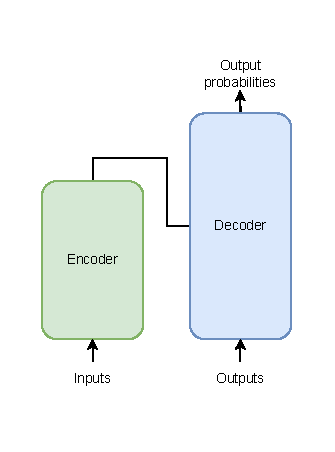
\includegraphics[width=0.5\linewidth]{Abschlussarbeit/Pictures/EncoderDecoder.pdf}
    \caption{Encoder Decoder}
    \label{fig:encoderDecoder}
\end{figure}

One of Transformer models key feature is that they are built with attention layers.
This special layer will tells the model to pay specific attention to certain words when representation each word in a sentence. 
If we consider for example a sentence \textit{A cat hunts a mouse, because she is hungry}.
A human would know immediate, that \textit{she} corresponds to \textit{the cat}. 



Where the mapping of a query and a set of key-value pairs, that are all vectors, to an output are described by an attention function.
A compatibility function of the query with the corresponding key determines the weight assigned to each value, which is then used to compute the generated outputs as a weighted sum of the values.
Every word of a sentence will get an embedding, that represents its meaning as well as a position-encoding, which gives information about the words position in the sentence.

An important technic that a transformer uses is called self-attention.
If we consider for example a sentence \textit{A cat hunts a mouse, because she is hungry}.
A human would know immediate, that \textit{she} corresponds to \textit{the cat}. 
A self-attention will consider every word of the sentence and know, the connection to the other words.
The model will learn that there is a connection between \textit{she} and \textit{cat},. 


\section{Transformer Models and its Application}
There are different models that are based on transformer. 
In the following we will introduce two different models.
On the one hand, we focus on {BERT}, which is the base of all models that are used during the experiments with in chapter \ref{exp}.
On the other hand, we introduce a \ac{GPT} which gained a lot of fame in the last years because of OpenAI's chat bot chatGPT.

\textbf{BERT} is an encoder model and uses only the encoder of a Transformer model. 
The attention layer can access all words in the initial sentence in each step.
Models like that are often characterized as having a bi-directional attention and are called auto-encoding models.

For tasks that require an understanding of the whole sentence, such as sentence classification, named entity recognition and extractive question answering are Encoder modlest best suited.

\textbf{GPT} is a decoder model and only uses the decoder of a Transformer model.
The attention layer can access only the words positioned before a given word in the sentence and are often called auto-regressive models.
Text generative tasks can be best suited with these models. 


